% move all configuration stuff into one file so we can focus on the content
\documentclass[aspectratio=169,hyperref={pdfpagelabels=false,colorlinks=true,linkcolor=white,urlcolor=lightblue},xcolor={table},t]{beamer}

%%%%%%%%%%%%%%%%%%%%%%%%%%%%%%%%%%%%%%%%%%%%%%%%%%%%%%%%%%%%%%%%%%%%%%%%%%%%%%%%%%
%%%%%%%%%%%%%%%%%%%%%%%%%%%%%%%%%%%%%%%%%%%%%%%%%%%%%%%%%%%%%%%%%%%%%%%%%%%%%%%%%%
% packages
\usepackage{pict2e}
\usepackage{epic}
\usepackage{amsmath,amsfonts,amssymb}
\usepackage{units}
\usepackage{fancybox}
\usepackage[absolute,overlay]{textpos} 
%\usepackage[table]{xcolor}
\usepackage{animate}
\usepackage{gensymb}
%\usepackage{graphicx}
%\usepackage{longtable}
\usepackage{multirow}
\usepackage{silence}
\usepackage{tikz}
\usepackage[backend=bibtex,style=ieee]{biblatex}
\AtEveryCitekey{\iffootnote{\tiny}{}}
%\addbibresource{include/references}



% fontsize
\let\Tiny=\tiny

%%%%%%%%%%%%%%%%%%%%%%%%%%%%%%%%%%%%%%%%%%%%%%%%%%%%%%%%%%%%%%%%%%%%%%%%%%%%%%%%%%
%%%%%%%%%%%%%%%%%%%%%%%%%%%%%%%%%%%%%%%%%%%%%%%%%%%%%%%%%%%%%%%%%%%%%%%%%%%%%%%%%%
% warnings
\pdfsuppresswarningpagegroup=1
\WarningFilter{biblatex}{Patching footnotes failed}
\WarningFilter{latexfont}{Font shape}
\WarningFilter{latexfont}{Some font shapes}
\WarningFilter{gensymb}{Not defining}


%%%%%%%%%%%%%%%%%%%%%%%%%%%%%%%%%%%%%%%%%%%%%%%%%%%%%%%%%%%%%%%%%%%%%%%%%%%%%%%%%%
%%%%%%%%%%%%%%%%%%%%%%%%%%%%%%%%%%%%%%%%%%%%%%%%%%%%%%%%%%%%%%%%%%%%%%%%%%%%%%%%%%
% theme & layout
\usetheme{Frankfurt}
\useinnertheme{rectangles}


%%%%%%%%%%%%%%%%%%%%%%%%%%%%%%%%%%%%%%%%%%%%%%%%%%%%%%%%%%%%%%%%%%%%%%%%%%%%%%%%%%
\setbeamertemplate{frametitle}[default][colsep=-4bp,rounded=false,shadow=false]
\setbeamertemplate{frametitle}
{%
    \nointerlineskip%
    %\vskip-0.5ex
    \begin{beamercolorbox}[wd=\paperwidth,ht=3.5ex,dp=0.6ex]{frametitle}
        \hspace*{1.3ex}\insertframetitle%
        
        \hspace*{1.3ex}\small\insertframesubtitle%
    \end{beamercolorbox}%
    \begin{textblock*}{100mm}(13.75cm,1cm)
        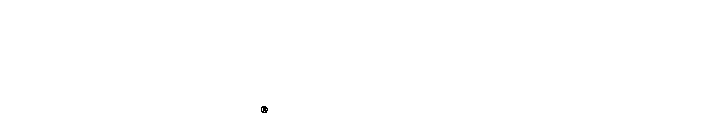
\includegraphics[height=.4cm,keepaspectratio]{../shared/Logo_GTCMT_white}
    \end{textblock*}
}


%%%%%%%%%%%%%%%%%%%%%%%%%%%%%%%%%%%%%%%%%%%%%%%%%%%%%%%%%%%%%%%%%%%%%%%%%%%%%%%%%%
\setbeamertemplate{title page}[default][colsep=-4bp,rounded=false,shadow=false]
\setbeamertemplate{title page}
{
    %\begin{textblock*}{100mm}(15cm,.51cm)
            %\href{https://github.com/alexanderlerch/ACA-Slides/blob/2nd_edition/\jobname.pdf}{\includegraphics[height=.5cm,keepaspectratio]{graph/Logo_github}}\hspace*{2ex}
    %\end{textblock*}
    %\begin{textblock*}{100mm}(15cm,1.3cm)
            %\href{\IEEELink}{\includegraphics[height=.5cm,keepaspectratio]{graph/icon/book}}\hspace*{2ex}
    %\end{textblock*}
    \vskip-10ex
    \begin{beamercolorbox}[wd=\paperwidth,ht=.7\paperheight,dp=0.6ex]{frametitle} %35ex
        %\begin{flushright}
            %\href{http://www.gtcmt.gatech.edu}{
\includegraphics[height=.8cm,keepaspectratio]{graph/Logo_GTCMT_black}}\hspace*{2ex}
        %\end{flushright}
        
        \hspace*{1.8ex}\LARGE\inserttitle%
        
        \vspace*{.5ex}
        
        \hspace*{1.3ex}\small\insertsubtitle%
        
        \vspace*{.5ex}
    \end{beamercolorbox}%
    \nointerlineskip%
    \begin{beamercolorbox}[wd=\paperwidth,ht=.4\paperheight,dp=0.6ex]{page number in head/foot}
        %\vspace*{-.5ex}
        \hspace*{1.7ex}\small\insertauthor%
        
        %\hspace*{1.7ex}\small }%
        
        \vspace*{12ex}
        \vfill
        \begin{flushright}
            \href{http://www.gtcmt.gatech.edu}{
\includegraphics[height=.5cm,keepaspectratio]{../shared/Logo_GTCMT_black}}\hspace*{2ex}
        \end{flushright}
    \end{beamercolorbox}%
}


%%%%%%%%%%%%%%%%%%%%%%%%%%%%%%%%%%%%%%%%%%%%%%%%%%%%%%%%%%%%%%%%%%%%%%%%%%%%%%%%%%
%\makeatother
\setbeamertemplate{footline}
{
  \leavevmode%
  \hbox{%
  \begin{beamercolorbox}[wd=.5\paperwidth,ht=2.25ex,dp=1ex,left,leftskip=1ex]{page number in head/foot}%
    \insertsubtitle
  \end{beamercolorbox}%
  \begin{beamercolorbox}[wd=.5\paperwidth,ht=2.25ex,dp=1ex,right,rightskip=1ex]{page number in head/foot}%
    \hfill
    \insertframenumber{} / \inserttotalframenumber
  \end{beamercolorbox}}%
  \vskip0pt%
}
%\makeatletter


%%%%%%%%%%%%%%%%%%%%%%%%%%%%%%%%%%%%%%%%%%%%%%%%%%%%%%%%%%%%%%%%%%%%%%%%%%%%%%%%%%
\beamertemplatenavigationsymbolsempty
\setbeamertemplate{navigation symbols}{}
\setbeamertemplate{blocks}[default]%[rounded=false,shadow=false]
\setbeamertemplate{itemize item}[square]
\setbeamertemplate{itemize subitem}[circle]
\setbeamertemplate{itemize subsubitem}[triangle]
\setbeamertemplate{enumerate item}[square]
\setbeamertemplate{enumerate subitem}[circle]
\setbeamertemplate{enumerate subsubitem}[circle]


%%%%%%%%%%%%%%%%%%%%%%%%%%%%%%%%%%%%%%%%%%%%%%%%%%%%%%%%%%%%%%%%%%%%%%%%%%%%%%%%%%
% colors
\setbeamercolor{structure}{fg=darkgray}
\setbeamercovered{transparent} %invisible
\setbeamercolor{bibliography entry author}{fg=black}
\setbeamercolor*{bibliography entry title}{fg=black}
\setbeamercolor*{bibliography entry note}{fg=black}
\setbeamercolor{frametitle}{fg=black}
\setbeamercolor{title}{fg=white}
\setbeamercolor{subtitle}{fg=white}
\setbeamercolor{frametitle}{fg=white}
\setbeamercolor{framesubtitle}{fg=white}
\setbeamercolor{mini frame}{fg=white, bg=black}
\setbeamercolor{section in head/foot}{fg=white, bg=darkgray}
\setbeamercolor{page number in head/foot}{fg=black, bg=gtgold}
\setbeamercolor{item projected}{fg=white, bg=black}

%---------------------------------------------------------------------------------

%%%%%%%%%%%%%%%%%%%%%%%%%%%%%%%%%%%%%%%%%%%%%%%%%%%%%%%%%%%%%%%%%%%%%%%%%%%%%%%%%%
%%%%%%%%%%%%%%%%%%%%%%%%%%%%%%%%%%%%%%%%%%%%%%%%%%%%%%%%%%%%%%%%%%%%%%%%%%%%%%%%%%
% title information
\title[]{MUSI6202: Digital Signal Processing for Music}   
\author[alexander lerch]{alexander lerch} 
%\institute{~}
%\date[Alexander Lerch]{}
%\titlegraphic{\vspace{-16mm}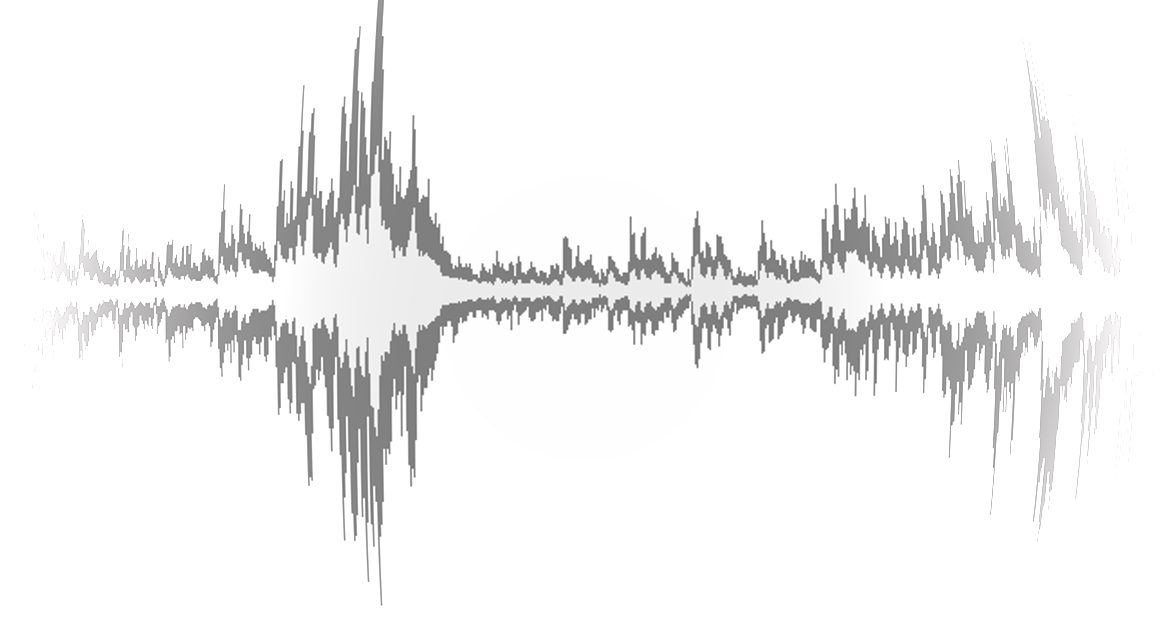
\includegraphics[width=\textwidth,height=3cm]{title}}

%%%%%%%%%%%%%%%%%%%%%%%%%%%%%%%%%%%%%%%%%%%%%%%%%%%%%%%%%%%%%%%%%%%%%%%%%%%%%%%%%%
%%%%%%%%%%%%%%%%%%%%%%%%%%%%%%%%%%%%%%%%%%%%%%%%%%%%%%%%%%%%%%%%%%%%%%%%%%%%%%%%%%
% colors
\definecolor{gtgold}{rgb}{.914, .664, 0} %0e7eed {rgb}{0.88,0.66,1,0.06} [234, 170, 0]/256 %96caff
\definecolor{darkgray}{rgb}{.15, .15, .15}
\definecolor{lightblue}{HTML}{0e7eed}
\definecolor{highlight}{rgb}{0, 0, 1} %_less!40

%%%%%%%%%%%%%%%%%%%%%%%%%%%%%%%%%%%%%%%%%%%%%%%%%%%%%%%%%%%%%%%%%%%%%%%%%%%%%%%%%%
%%%%%%%%%%%%%%%%%%%%%%%%%%%%%%%%%%%%%%%%%%%%%%%%%%%%%%%%%%%%%%%%%%%%%%%%%%%%%%%%%%
% relative paths
\graphicspath{{../graph/}}


%%%%%%%%%%%%%%%%%%%%%%%%%%%%%%%%%%%%%%%%%%%%%%%%%%%%%%%%%%%%%%%%%%%%%%%%%%%%%%%%%%
%%%%%%%%%%%%%%%%%%%%%%%%%%%%%%%%%%%%%%%%%%%%%%%%%%%%%%%%%%%%%%%%%%%%%%%%%%%%%%%%%%
% units
\setlength{\unitlength}{1mm}

%%%%%%%%%%%%%%%%%%%%%%%%%%%%%%%%%%%%%%%%%%%%%%%%%%%%%%%%%%%%%%%%%%%%%%%%%%%%%%%%%%
%%%%%%%%%%%%%%%%%%%%%%%%%%%%%%%%%%%%%%%%%%%%%%%%%%%%%%%%%%%%%%%%%%%%%%%%%%%%%%%%%%
% math
\DeclareMathOperator*{\argmax}{argmax}
\DeclareMathOperator*{\argmin}{argmin}
\DeclareMathOperator*{\atan}{atan}
\DeclareMathOperator*{\arcsinh}{arcsinh}
\DeclareMathOperator*{\sign}{sign}
\DeclareMathOperator*{\tcdf}{tcdf}
\DeclareMathOperator*{\si}{sinc}
\DeclareMathOperator*{\princarg}{princarg}
\DeclareMathOperator*{\arccosh}{arccosh}
\DeclareMathOperator*{\hwr}{HWR}
\DeclareMathOperator*{\flip}{flip}
\DeclareMathOperator*{\sinc}{sinc}
\DeclareMathOperator*{\floor}{floor}
\newcommand{\e}{{e}}
\newcommand{\jom}{\mathrm{j}\omega}
\newcommand{\jOm}{\mathrm{j}\Omega}
\newcommand   {\mat}[1]    		{\boldsymbol{\uppercase{#1}}}		%bold
\renewcommand {\vec}[1]    		{\boldsymbol{\lowercase{#1}}}		%bold

%%%%%%%%%%%%%%%%%%%%%%%%%%%%%%%%%%%%%%%%%%%%%%%%%%%%%%%%%%%%%%%%%%%%%%%%%%%%%%%%%%
%%%%%%%%%%%%%%%%%%%%%%%%%%%%%%%%%%%%%%%%%%%%%%%%%%%%%%%%%%%%%%%%%%%%%%%%%%%%%%%%%%
% media9
\newcommand{\includeaudio}[1]{
\href{run:audio/#1.mp3}{
\includegraphics[width=5mm, height=5mm]{graph/SpeakerIcon}}}

\newcommand{\includeanimation}[4]{{\begin{center}
                        \animategraphics[autoplay,loop,scale=.7]{#4}{animation/#1-}{#2}{#3}        
                        \end{center}
                        \addreference{matlab source: \href{https://github.com/alexanderlerch/ACA-Plots/blob/master/matlab/animate#1.m}{matlab/animate#1.m}}}
                        \inserticon{video}}
                        
%%%%%%%%%%%%%%%%%%%%%%%%%%%%%%%%%%%%%%%%%%%%%%%%%%%%%%%%%%%%%%%%%%%%%%%%%%%%%%%%%%
%%%%%%%%%%%%%%%%%%%%%%%%%%%%%%%%%%%%%%%%%%%%%%%%%%%%%%%%%%%%%%%%%%%%%%%%%%%%%%%%%%
% other commands
\newcommand{\question}[1]{%\vspace{-4mm}
                          \setbeamercovered{invisible}
                          \begin{columns}[T]
                            \column{.9\textwidth}
                                \textbf{#1}
                            \column{.1\textwidth}
                                \vspace{-8mm}
                                \begin{flushright}
                                     
\includegraphics[width=.9\columnwidth]{graph/question_mark}
                                \end{flushright}
                                \vspace{6mm}
                          \end{columns}\pause\vspace{-12mm}}

\newcommand{\toremember}[1]{
                        \inserticon{lightbulb}
                        }

\newcommand{\matlabexercise}[1]{%\vspace{-4mm}
                          \setbeamercovered{invisible}
                          \begin{columns}[T]
                            \column{.8\textwidth}
                                \textbf{matlab exercise}: #1
                            \column{.2\textwidth}
                                \begin{flushright}
                                     \includegraphics[scale=.5]{graph/logo_matlab}
                                \end{flushright}
                                %\vspace{6mm}
                          \end{columns}}

\newcommand{\addreference}[1]{  
                  
                    \begin{textblock*}{\baselineskip }(.98\paperwidth,.5\textheight) %(1.15\textwidth,.4\textheight)
                         \begin{minipage}[b][.5\paperheight][b]{1cm}%
                            \vfill%
                             \rotatebox{90}{\tiny {#1}}
                        \end{minipage}
                   \end{textblock*}
                    }
                    
\newcommand{\figwithmatlab}[1]{
                    \begin{figure}
                        \centering
                        \includegraphics[scale=.7]{#1}
                        %\label{fig:#1}
                    \end{figure}
                    
                    \addreference{matlab source: \href{https://github.com/alexanderlerch/MUSI-6202/blob/main/matlab/plot#1.m}{plot#1.m}}}
\newcommand{\figwithref}[2]{
                    \begin{figure}
                        \centering
                        \includegraphics[scale=.7]{#1}
                        \label{fig:#1}
                    \end{figure}
                    
                    \addreference{#2}}  
                                    
\newcommand{\inserticon}[1]{
                    \begin{textblock*}{100mm}(14.5cm,7.5cm)
                        \includegraphics[height=.8cm,keepaspectratio]{graph/#1}
                    \end{textblock*}}            

%%%%%%%%%%%%%%%%%%%%%%%%%%%%%%%%%%%%%%%%%%%%%%%%%%%%%%%%%%%%%%%%%%%%%%%%%%%%%%%%%%
%%%%%%%%%%%%%%%%%%%%%%%%%%%%%%%%%%%%%%%%%%%%%%%%%%%%%%%%%%%%%%%%%%%%%%%%%%%%%%%%%%
% counters
\newcounter{i}
\newcounter{j}
\newcounter{iXOffset}
\newcounter{iYOffset}
\newcounter{iXBlockSize}
\newcounter{iYBlockSize}
\newcounter{iYBlockSizeDiv2}
\newcounter{iXBlockSizeDiv2}
\newcounter{iDistance}

\newcommand{\IEEELink}{https://ieeexplore.ieee.org/servlet/opac?bknumber=9965970}

\addbibresource{../shared/references}



\subtitle{Part 18: Sample Rate Conversion (SRC)}

%%%%%%%%%%%%%%%%%%%%%%%%%%%%%%%%%%%%%%%%%%%%%%%%%%%%%%%%%%%%%%%%%%%%%%%%%%%%
\begin{document}
    % generate title page
	\title[]{Digital Signal Processing for Music}   
\author[alexander lerch]{alexander lerch} 
%\institute{~}
%\date[Alexander Lerch]{}
\titlegraphic{\vspace{-16mm}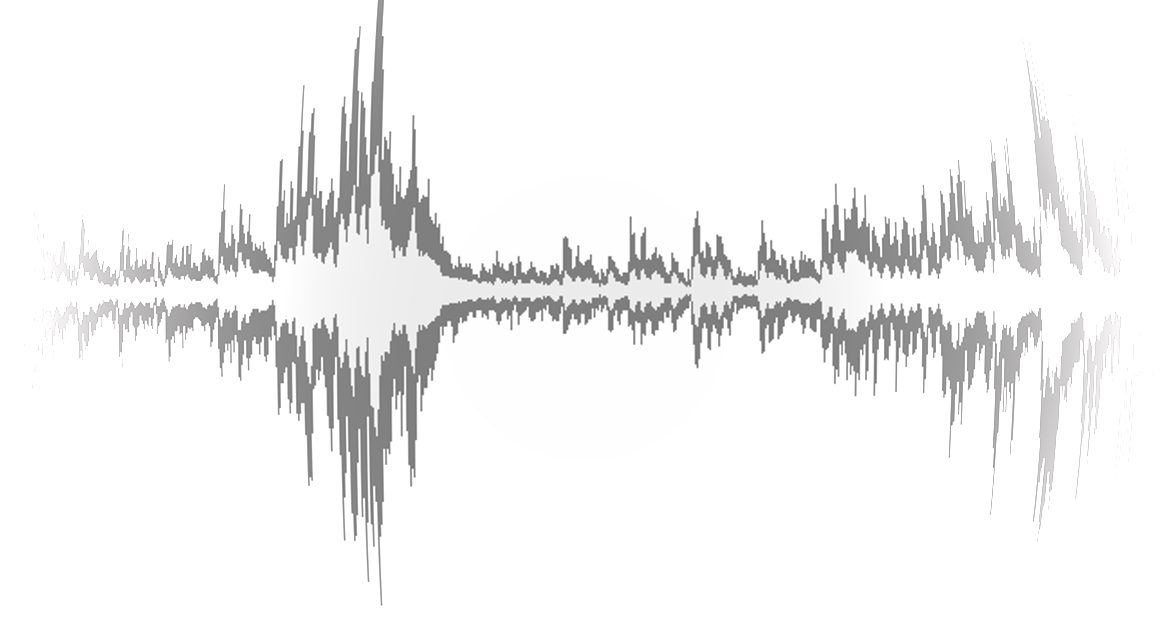
\includegraphics[width=\textwidth,height=3cm]{title}}


\begin{frame}
    \titlepage
    %\vspace{-5mm}
    \begin{flushright}
        \href{http://www.gtcmt.gatech.edu}{
\includegraphics[height=.8cm,keepaspectratio]{../shared/Logo_GTCMT_black}}
    \end{flushright}
\end{frame}


\section[intro]{introduction}
	\begin{frame}{sample rate conversion}{introduction }
        \vspace{-3mm}
        \begin{block}{sample rate conversion}
            WP:''changing the sampling rate of a discrete signal to obtain a new discrete representation of the underlying continuous signal.''
        \end{block}
        \bigskip
        \only<1>{
            \figwithmatlab{SRC}
        }
        \only<2>{
            \bigskip
            \textbf{typical applications}
                \begin{itemize}
                    \item   audio file/media conversion
                    \item   word clock synchronization (multiple devices)
                    \item   DJing/scratching
                \end{itemize}
        }
        \vspace{30mm}    
	\end{frame}

	\begin{frame}{sample rate conversion}{introduction}
        \begin{itemize}
            \item   \textbf{terminology}
                \begin{itemize}
                    \item   \textit{synchronous} resampling
                        \begin{itemize}
                            \item   clock rates are coupled
                            \item   resampling factor stays constant
                        \end{itemize}
                    \pause
                    \item   \textit{asynchronous} resampling
                        \begin{itemize}
                            \item   clock rates are independent
                            \item   resampling factor may change
                        \end{itemize}
                \end{itemize}
            \bigskip
            \item   \textbf{ideal result}
                \begin{itemize}
                    \item   spectrum in the used band unchanged
                    \item   spectral periodicity (determined by sample rate) changed
                \end{itemize}
        \end{itemize}
    \end{frame}

        \section{inserting \& removing zeros}
	\begin{frame}{sample rate conversion}{upsampling by inserting zeros}
        \vspace{-3mm}
        \begin{itemize}
            \item   task: \textbf{upsample by integer factor} $L$
            \pause 
            \begin{enumerate}
                \item   insert $L-1$ zeros between all samples
                \item   apply anti-imaging filter
            \end{enumerate}
        \end{itemize}
        \only<3>{
		\begin{figure}
            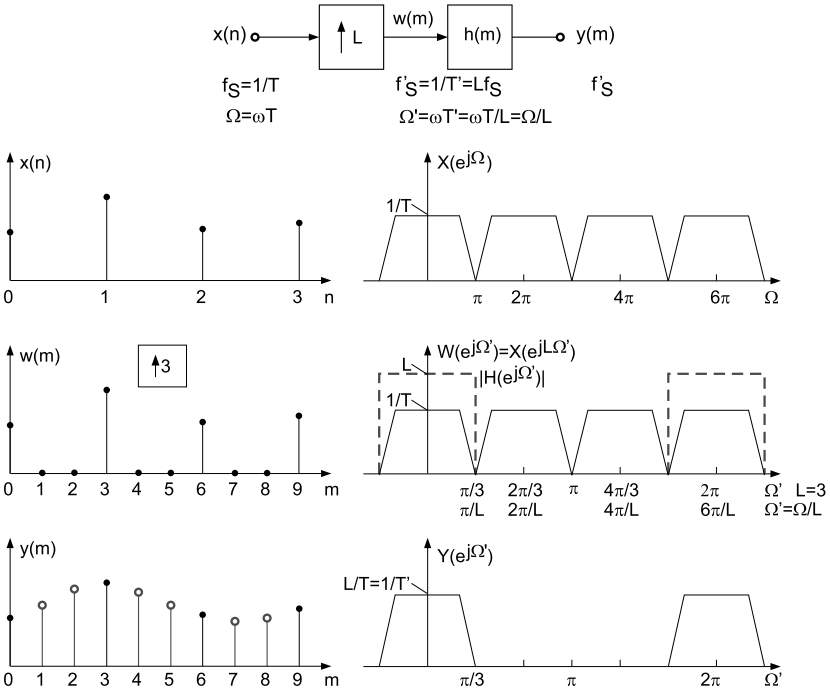
\includegraphics[scale=0.29]{Graph/upsampling_zeros}
		\end{figure}
        }
    \end{frame}
	\begin{frame}{sample rate conversion}{downsampling by removing samples}
        \vspace{-3mm}
        \begin{itemize}
            \item   task: \textbf{downsample by integer factor} $M$
            \pause 
            \begin{enumerate}
                \item   apply anti-aliasing filter
                \item   take every $M$th sample
            \end{enumerate}
        \end{itemize}
        \only<3>{
		\begin{figure}
            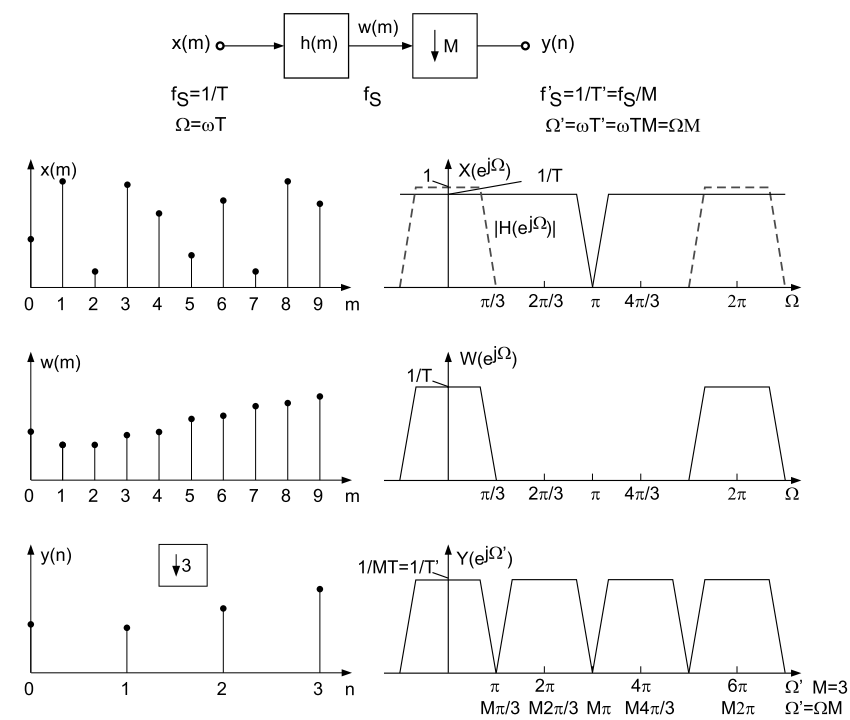
\includegraphics[scale=0.29]{Graph/downsampling_remove}
		\end{figure}
        }
    \end{frame}
	\begin{frame}{sample rate conversion}{resampling by rational factor}
        \begin{itemize}
            \item   task: \textbf{convert sample rate to any} other (coupled) sample rate
            \pause 
            \begin{enumerate}
                \item   convert sample rate ratio to integer factors\\ e.g.:  \nicefrac{48}{44.1} $\Rightarrow$ $L=160, M=147$
                \pause
                \item   insert zeros
                \item   apply anti-imaging filter
                \pause
                \item   apply anti-aliasing filter (filters can be combined)
                \item   remove samples
            \end{enumerate}
        \end{itemize}
        \bigskip
		\only<4->{
        \begin{figure}
            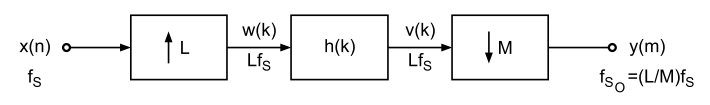
\includegraphics[scale=0.5]{Graph/resampling_flow}
		\end{figure}
        }
        \vspace{50mm}
    \end{frame}
        \section{sinc}
	\begin{frame}{sample rate conversion}{sinc interpolation 1/2}
        \begin{itemize}
            \item   perfect reconstruction of the sampled spectrum is possible with ideal filter
            \item   [$\Rightarrow$] resampling should be possible by time domain convolution with $\sinc$
        \end{itemize}
        \only<1>{
        \begin{figure}
                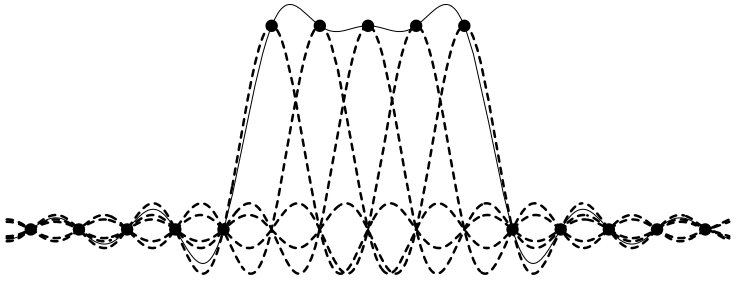
\includegraphics[scale=0.4]{Graph/src_sincinterpol}
        \end{figure}
        }
            \pause
            \begin{equation*}
                x(i-\alpha) = \sum\limits_{m=-\infty}^{\infty}x(m)\frac{\Omega_C}{\pi}\frac{sin\left(\Omega_C(i-\alpha-m)\right)}{\Omega_C(i-\alpha-m)}
            \end{equation*}
            $\Omega_C$ is the cutoff frequency of the  ideal lowpass
        \visible<2>{
        \begin{figure}
                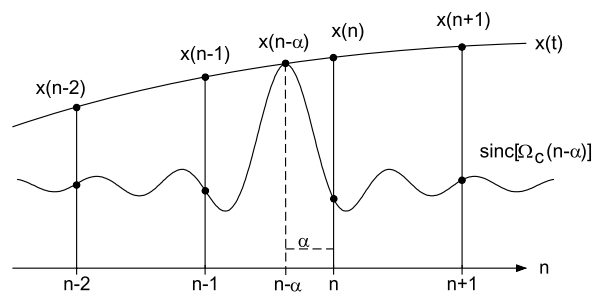
\includegraphics[scale=0.4]{Graph/resample_sinc}
        \end{figure}
        }
    \end{frame}
	\begin{frame}{sample rate conversion}{sinc interpolation 2/2}
        \begin{itemize}
            \item   practical implementation: \textbf{windowed sinc}
        \end{itemize}
    \end{frame}

\section{other interpolation}
	\begin{frame}{sample rate conversion}{polynomial interpolation}
        \begin{itemize}
            \item   \textbf{interpolation methods }
                \begin{itemize}
                    \item   can be interpreted as filters with time-variant filter coefficients
                    \item   not based on traditional filter desing methods
                \end{itemize}
            \bigskip
            \item<2->   polynomial interpolation
                \begin{eqnarray*}
                    f(t) &=& \sum\limits_{k=0}^\mathcal{O}x_k p_k(t)\\
                    p_k(t) &=& \prod\limits_{j=0}^\mathcal{O}\frac{t-t_j}{t_k-t_j}
                \end{eqnarray*}
        \end{itemize}
    \end{frame}
	\begin{frame}{sample rate conversion}{polynomial interpolation example}
        \vspace{-5mm}
        \begin{footnotesize}
        \begin{eqnarray*}
            x(t) &=& \frac{1}{t}\\
            \text{nodes: } t &=& [2, 4, 5]\\
            \pause
            p_0(t) &=& \frac{(t-4)(t-5)}{(2-4)(2-5)} = \frac{(t-4)(t-5)}{6}\\
            p_1(t) &=& \frac{(t-2)(t-5)}{(4-2)(4-5)} = -\frac{(t-2)(t-5)}{2}\\
            p_2(t) &=& \frac{(t-2)(t-4)}{(5-2)(5-4)} = \frac{(t-2)(t-4)}{3}\\
            \pause
             f(t) &=& \sum\limits_{k=0}^\mathcal{O}x_k p_k(t)\\
            \pause
            \Rightarrow f(t) &=& p_0\frac{1}{2}+p_1\frac{1}{4}+p_2\frac{1}{5}\\
            &=& 0.025t^2 - 0.275t + 0.95 .
        \end{eqnarray*}
        \end{footnotesize}
    \end{frame}
	\begin{frame}{sample rate conversion}{polynomial interpolation example}
        \figwithmatlab{PolyInterp}
    \end{frame}
	\begin{frame}{sample rate conversion}{special case: linear interpolation}
        \begin{itemize}
            \item   1st order $\rightarrow$ 2 points
        \end{itemize}
        \begin{footnotesize}
        \begin{eqnarray*}
            x(t) &=& \frac{1}{t}\\
            \text{nodes: } t &=& [2, 4]\\
            \pause
            p_0(t) &=& \frac{(t-4)}{(2-4)} = \frac{(4-t)}{2}\\
            p_1(t) &=& \frac{(t-2)}{(4-2)} = \frac{(t-2)}{2}\\
            \pause
             f(t) &=& \sum\limits_{k=0}^\mathcal{O}x_k p_k(t)\\
            \pause
            \Rightarrow f(t) &=& p_0\frac{1}{2}+p_1\frac{1}{4}\\
            &=& - \frac{1}{8}t + \frac{3}{4}.
        \end{eqnarray*}
         \end{footnotesize}
    \end{frame}
	\begin{frame}{sample rate conversion}{special case: linear interpolation}
        \begin{figure}
            \begin{center}
                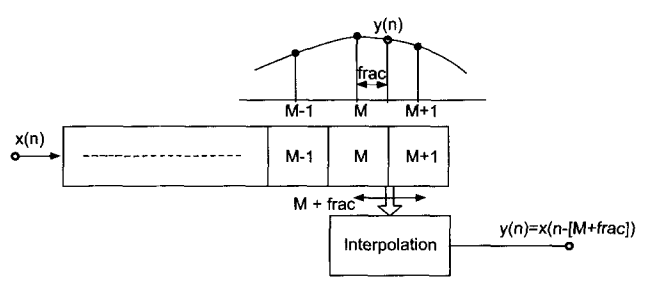
\includegraphics[scale=0.4]{Graph/src_lininterpol}
            \end{center}
        \end{figure}
        
        \begin{equation*}
            \hat{x} = x_l\cdot (1-frac) + x_r\cdot frac
        \end{equation*}
    \end{frame}
	\begin{frame}{sample rate conversion}{interpolation comparison}
        \begin{figure}
            \hspace*{-5mm}
            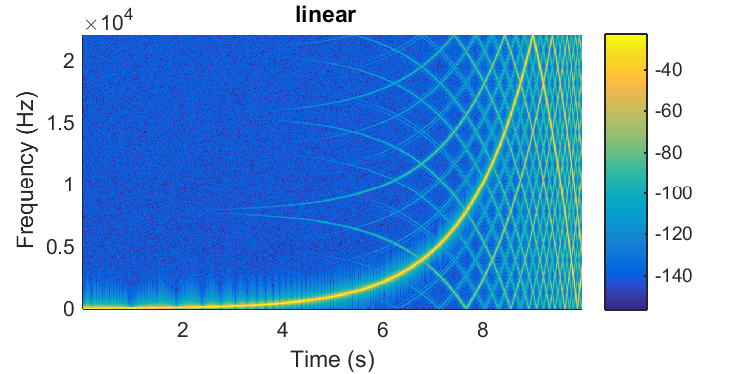
\includegraphics[scale=.5]{graph/src_sine_1}
            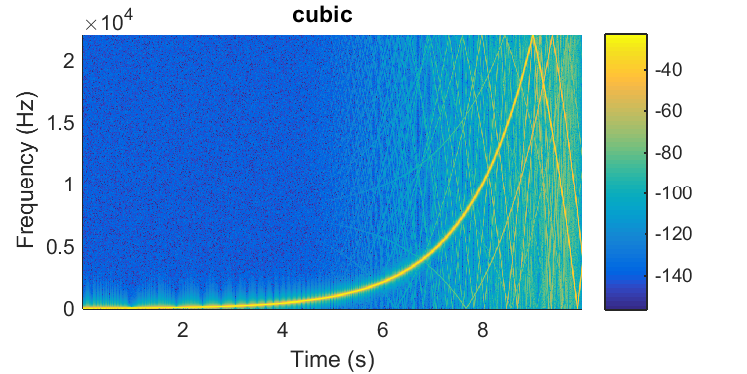
\includegraphics[scale=.5]{graph/src_sine_2}

            \hspace*{-5mm}
            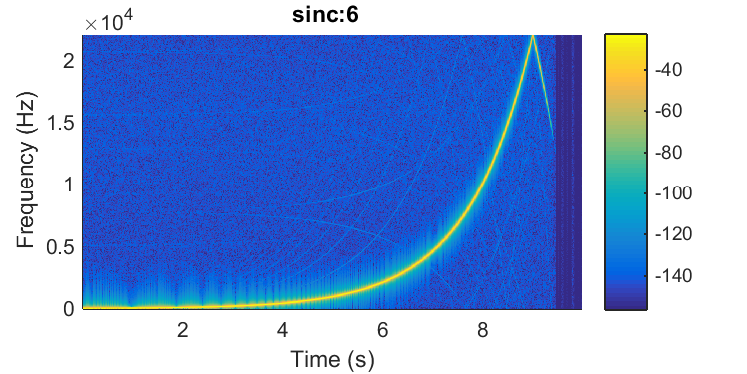
\includegraphics[scale=.5]{graph/src_sine_3}
            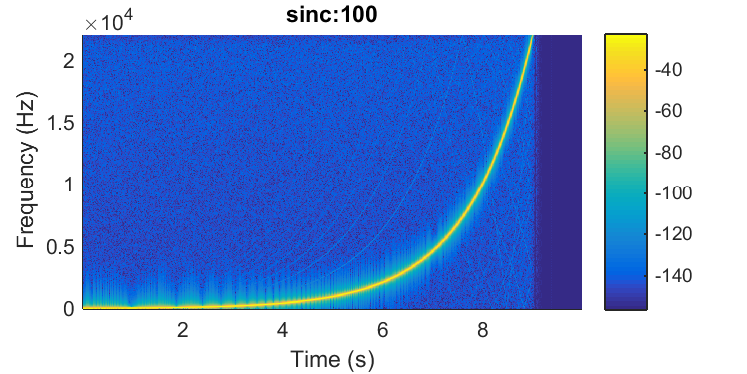
\includegraphics[scale=.5]{graph/src_sine_4}
        \end{figure}
	\end{frame}
	\begin{frame}{sample rate conversion}{downsampling audio examples}
        \begin{footnotesize}
		\begin{table}
			\begin{center}
				\begin{tabular}{lcccccc}
                 & orig (\unit[48]{kHz}) & ds (\unit[6]{kHz}, w/o filt) & ds (\unit[6]{kHz}, w/ filt)\\\hline
                sax& \includeaudio{alto-sax} & \includeaudio{alto-saxds8}  & \includeaudio{alto-saxds8_proper} \\
                big band& \includeaudio{bigband} & \includeaudio{bigbandds8}  & \includeaudio{bigbandds8_proper} \\
				\end{tabular}  
			\end{center}
		\end{table}
        \end{footnotesize}
	\end{frame}
	
\section{summary}
		\begin{frame}{sample rate conversion}{summary}
            \begin{itemize}
                \item   resampling: estimate different sample points of underlying continuous signal
                \smallskip
                \item   as with sampling, proper filtering has to take place
                \smallskip
                \item   some interpolation approaches have filter ``built-in''
                \smallskip
                \item   perfect reconstruction impossible (infinite sinc), however, perceptually artifact-free resampling is possible
                    \begin{itemize}
                        \item   main issue: filter cut-off and steepness vs.\ aliasing
                    \end{itemize}
            \end{itemize}
 		\end{frame}

\end{document}

